\documentclass[12pt, twoside, a4paper]{article}

\usepackage[utf8]{inputenc}
\usepackage[english]{babel}
\usepackage{csquotes}

\usepackage[margin=1in,left=1.5in,includefoot, a4paper]{geometry}

\usepackage{pythonhighlight}
\usepackage{listings}

% Python style for highlighting
\newcommand\pythonstyle{\lstset{
language=Python,
basicstyle=\ttm,
otherkeywords={self},             % Add keywords here
keywordstyle=\ttb\color{deepblue},
emph={MyClass,__init__},          % Custom highlighting
emphstyle=\ttb\color{deepred},    % Custom highlighting style
stringstyle=\color{deepgreen},
frame=tb,                         % Any extra options here
showstringspaces=false            % 
}}

% Python environment
\lstnewenvironment{ipython}[1][]
{
\pythonstyle
\lstset{#1}
}
{}

% Header and Footer
\usepackage{fancyhdr}
\pagestyle{fancy}
\fancyfoot{}
\fancyhead{}
\renewcommand{\headrulewidth}{0pt}
\fancyfoot[LE]{\thepage}
\fancyfoot[RO]{\thepage}
%\fancyfoot[LE,RO]{\thepage}

% Custom colors
\usepackage{color}
\definecolor{deepblue}{rgb}{0,0,0.5}
\definecolor{deepred}{rgb}{0.6,0,0}
\definecolor{deepgreen}{rgb}{0,0.5,0}

\usepackage{xcolor} % For highlighting changes

\usepackage{graphicx}
\usepackage{subfig}
\usepackage{float}

\usepackage{pgfgantt}

\usepackage{biblatex}

\addbibresource{references.bib}

\begin{document}

\begin{titlepage}
    \begin{center}
        \vspace*{.06\textheight}{\scshape\LARGE Birkbeck, University of London\par}\vspace{1.5cm} % University name
        \rule[0.5ex]{\linewidth}{2pt}\vspace*{-\baselineskip}\vspace*{3.2pt}
        \rule[0.5ex]{\linewidth}{1pt}\\[\baselineskip]
        \huge{\bfseries Pneumonia Detection from Chest X-Ray Images}\\[4mm]
        \rule[0.5ex]{\linewidth}{1pt}\vspace*{-\baselineskip}\vspace{3.2pt}
        \rule[0.5ex]{\linewidth}{2pt}\\
        [1.5cm]


        \begin{minipage}[t]{0.4\textwidth}
        \begin{flushleft} \large
        \emph{Author:}\\
        {Baran Buluttekin} % Author name - remove the \href bracket to remove the link
        \end{flushleft}
        \end{minipage}
        \begin{minipage}[t]{0.4\textwidth}
        \begin{flushright} \large
        \emph{Supervisor:} \\
        {Dr. George Magoulas} % Supervisor name - remove the \href bracket to remove the link  
        \end{flushright}
        \end{minipage}\\
        [2cm] %[3cm]
        
\includegraphics[scale=0.05]{img/birkbeck-shield.png}
            \vfill

            \large \textit{A project proposal submitted in fulfillment of the requirements\\ for the degree of MSc Data Science}\\[0.3cm] % University requirement text
            \textit{in the}\\[0.4cm]
            Department of Computer Science\\[2cm] % Research group name and department name
 
            \vfill

            {\large \today}\\[4cm] % Date
            %\includegraphics{Logo} % University/department logo - uncomment to place it
 
            \vfill
    \end{center}
\end{titlepage}    
\thispagestyle{empty}
\cleardoublepage

\pagenumbering{roman}

\section*{Declaration}
\addcontentsline{toc}{section}{Declaration}

\vfill
\textit{I have read and understood the sections of plagiarism in the College Policy on assessment offences and confirm that the work is my own, with the work of others clearly acknowledged. I give my permission to submit my report to the plagiarism testing database that the College is using and test it using plagiarism detection software, search engines or meta- searching software.}
\vfill

\clearpage

\section*{Abstract}
\addcontentsline{toc}{section}{Abstract}
This Data Science project will be focusing on classification of X-ray images labelled based on patients with or without pneumonia. This proposal document will outline logistics and decisions made for the project in sequential order. \textcolor{blue}{Section one, two and three introduce background information about the project.} First section of the proposal will give general facts about pneumonia and highlight important details about the related work carried out within the industry. More specifically related pneumonia detection research will be examined and how this research effected decisions of this project. Second section of the proposal will give reasoning of the dataset of choice and explains why this specific dataset is chosen amongst others. Section third will give a quick introduction to artificial neural networks (ANN's) and some background information about the benchmark neural network architectures as well as answers the question of why this specific machine learning field is chosen. Section 4 will give clear definition for the aim and objectives of this project. \textcolor{blue}{Section five details each objectives and explains how they will be implemented.} Sixth section list the tools and techniques considered to be used and some brief reasoning behind them. Lastly, final section will layout time frame for the execution of the project. 

\clearpage

\tableofcontents
\thispagestyle{empty}
\cleardoublepage
    

\pagenumbering{arabic}
\setcounter{page}{1}


\section{Introduction}

Pneumonia is swelling (inflammation) of the tissue in one or both lungs. It is usually formed at the end of breathing tubes of the lungs and cause these tubes to inflame and fill up with fluid. In the UK, pneumonia effects around 8 in 1000 adults each year \cite{nhs}. Global economic cost of pneumonia has estimated at \$17 billion annually \cite{cost}. Currently detecting pneumonia cases heavily relies on chest X-ray image examination which requires expert radiologists to diagnose. Building intelligent system to diagnose the pneumonia can help  health care services to increase efficiency, reduce costs and could help increase early diagnoses in countries with inadequate access to health care.

\subsection{Related work}

There are number of research has been published about lung diseases related detection. Most prevalent ones are the CheXNet \cite{CheXNetRP} and ChestX-ray8 \cite{ChestX-ray8}, both of these research carried out by training on same dataset ChestX-ray8 \cite{ChestX-ray8}. ChestX-ray8 comprises of approximately 100,000 frontal view chest X-ray images labelled by extracting information from the accompanied radiologists notes with using variety of different NLP (Natural language processing) techniques from the openi\cite{openi} database. ChestX-ray8 authored by researchers from National Institute of Health (NIH) and published at 2018.
Most profound effect of this paper is the creation of the ChestX-ray8 dataset which has become one of the widely used dataset in computer vision research related to lung diseases. More detailed information about the dataset can be found in dataset section of this proposal. 

CheXNet is another related article authored by researchers from Stanford University ML group. Prediction of lung diseases achieved by 121 layer convolutional neural network and designed to predict 14 pathologies in the ChestX-ray8 dataset. One of the major importance of this paper is the setting the setting benchmark for human level detection for chest X-ray images. One of the most fundamental difference of the X-ray related disease prediction is the definition of human level accuracy. Due to the nature of required expertise in X-ray images leaves general public out of the scope when it comes to human level performance of these pathologies. Anyone who have not been trained in radiology will not be able to detect any lung diseases in the Chest X-ray images. For example the image below is sample of two chest X-ray images almost indistinguishable to general audience.

\begin{figure}[H]%
    \centering
    \subfloat{{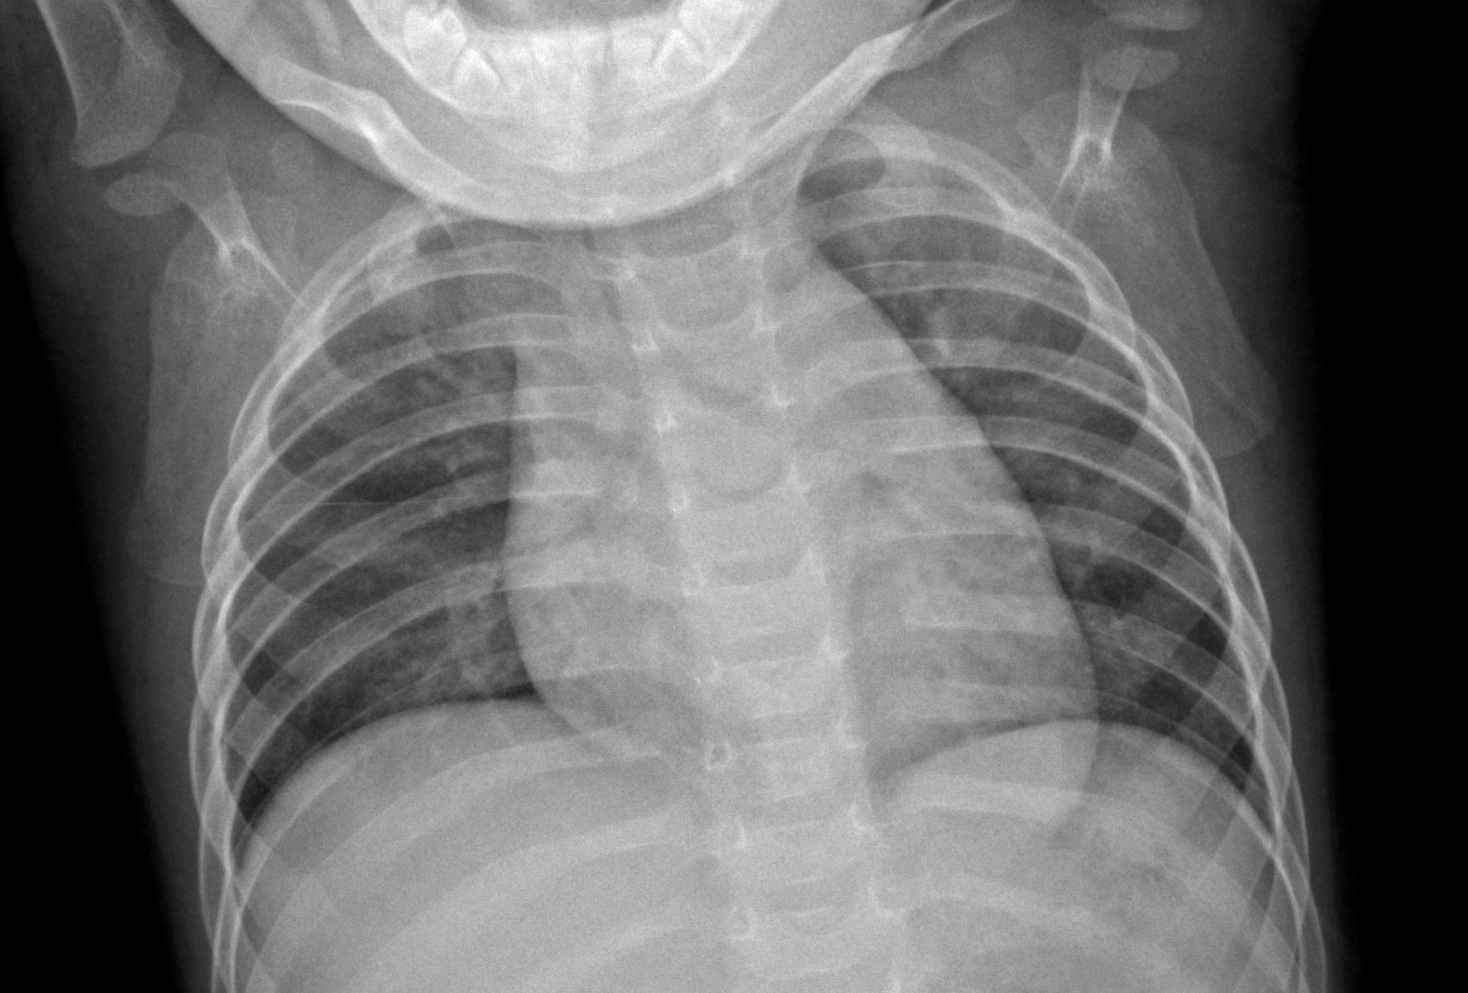
\includegraphics[width=.4\textwidth]{img/chest_xray_train_NORMAL_IM-0133-0001.jpeg} }}%
    \qquad
    \subfloat{{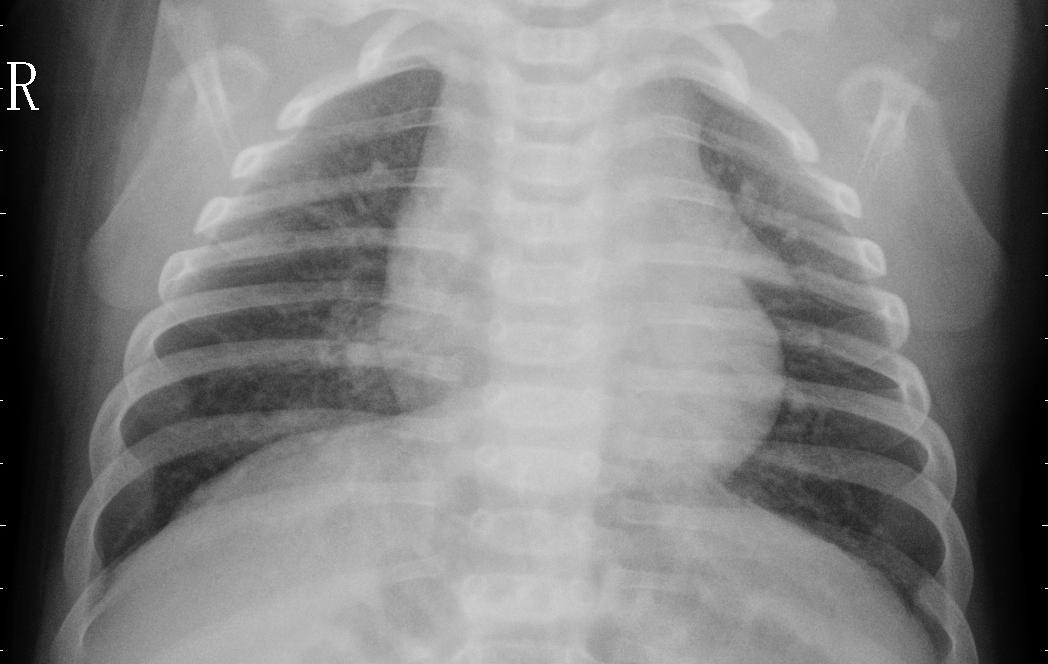
\includegraphics[width=.4\textwidth]{img/chest_xray_train_PNEUMONIA_person1007_virus_1690.jpeg} }}%
    \caption{Two sample X-ray Chest images.}%
    \label{fig:sample}%
\end{figure}
Given this challenge authors of the CheXNet conduct a test to establish benchmark for radiologists. They have collected 420 frontal chest X-rays and asked practicing radiologists in Stanford University to label them for all 14 pathologies. Radiologists selected with different range of experience, and had 4, 7, 25 and 28 years of experience. X-ray images presented to radiologists without any patient information or any symptoms experienced by patients and their diagnoses predictions measured based on underlying state of the X-ray patients. Fallowing is the table showing the summary statistic of this test for the 4 radiologists participated to test on F1 score, which is harmonic average of precision and recall.\cite{CheXNetRP}:
\begin{table}[h!]
    \centering
     \begin{tabular}{l r} 
     \hline
      & F1 Score (95\% CI) \\ [0.5ex] 
     \hline
     Radiologists 1 & 0.383 (0.309, 0.453) \\ 
     Radiologists 2 & 0.356 (0.282, 0.428) \\
     Radiologists 2 & 0.365 (0.291, 0.435) \\
     Radiologists 4 & 0.442 (0.390, 0.492) \\
     \hline
     Radiologists Avg & 0.387 (0.330, 0.442) \\ [1ex] 
     \hline
     \end{tabular}
     \caption{Radiologist prediction performances from CheXNet.}
     \label{table:radiologist}
\end{table}

Importance of this test is that it gives us a rough estimate for human level accuracy benchmark to assess the model performance for new detection models.


\clearpage
\section{Dataset}
Choosing and processing dataset have a crucial importance on success of the any machine learning task. There are several dataset available online that relate to chest X-Ray images. Given the large number of choices for selecting the dataset there are few criteria important to check while deciding the final dataset.

\subsection{General guidelines while deciding on the dataset}
In this section I have highlighted my reasons for deciding on the dataset of choice for this research project. Main points for decision are:
\begin{enumerate}
    \item \textbf{Reproducibility: }Dataset of choice must allow reader to reproduce the work in order to assess all the points discussed in the report. That would require dataset to be public.
    \item \textbf{Labelling: }Dataset must contain labels of patients state. Such as being diagnosed with pneumonia or not.
    \item \textbf{License: }Dataset should have a license that permits research.
\end{enumerate}
I will be evaluating dataset available while considering general guidelines outlined above.

\subsection{OpenI database}

OpenI\cite{openi} is a database that is service of National Library of Medicine. It enables search for medical images, graphs and charts through text as well as image query. As of writing of this proposal it has over 3.7 million images, and 3,955 radiology reports. It is the main source for ChestX-ray8 dataset mentioned previously in Related Work section. Despite the fact it contains very large data for chest X-rays, this source is not suitable for this project due to the fact that images does not includes labels for the patients state (e.g., Pneumonia or normal). Chest X-ray data in this database is the image accompanied by radiologist report which is advisory document. Mainly because the lack of labels this dataset is not suitable for this project where the choice will be a supervised classification task.

\subsection{ChestX-ray8}
This dataset created part of the ChestX-ray8\cite{ChestX-ray8} paper (Also known as ChestX-ray14). Original source of this dataset is OpenI\cite{openi} medical database as mentioned in previous subsection. Authors first short-listed eight common thoracic pathologies subsequently related X-rays searched from the database based on these pathology keywords. Most positive quality of this dataset amongst the other options is the sheer quantity of the data points which is by far the largest in size. This attribute especially important when it comes to certain computer vision techniques such as Neural Networks due to the fact that large datasets increases the variance and enables better generalization. Despite this positive points, quality of the labelling of this dataset has come to questioning by radiologists\cite{counterray8}. Due to this considerable labelling inconsistencies this dataset have not been chosen for this project.

\subsection{Cell press research}
Shortcomings of first two datasets compelled me to searched further for new dataset that does not have the problems I point out previously. Research from Cell Press\cite{dataset}, together with the data that made public, provided a solution to these problems. Dataset the team released contains 5856 hand labelled X-ray chest images from children aged between one to five years old. X-ray images collected as part of the routine clinical care at the Guangzhou Women and Children’s Medical Center, Guangzhou, China. All images screened for quality control and low quality or unreadable x-rays discarded. Labels of the images also checked by two expert physician and only approved images included in the dataset. Finally this dataset released under Creative Commons license Attribution 4 (CC BY 4.0) that allow copy, distribution of the material as well as transform and building upon material for any purposes. In light of all these attributes I choose this dataset for my project.

\clearpage

\section{Computer Vision}
Importance of X-ray image analysis in pneumonia diagnoses clearly highlights that this is a computer vision problem. In essence computer vision is a scientific field aims to automate vision task usually performed by humans. Vision on earth begin approximately 543 million years ago when trilobites developed basic vision system \cite{firstvision}. Development of vision helped increase the specie variation and development on earth significantly in respect to reproduction, finding food and many other reasons. Largely due to this very important nature of vision, research in how vision performed in species and how to automate the vision task gained a lot of attraction. Early research in this field inspired by the biological vision system. More specifically model of mammal neural system in respect to vision was the center point. In 1959 experiment on cat visual system by Hubel and Wiesel \cite{hubel:single} highlighted the inner functioning of vision by discovering effect of dark edges causing activation in visual cortex. They also concluded that visual cortex passing this signals from detected edges to later centers of the brain where those edges are combined to represent more complex shapes. This idea of simple to more complex neural structure inspired Japanese computer scientist Kunihiko Fukushima to propose system he called \textit{Neocognitron} \cite{fukushima:neocognitronbc}. In the article he laid out simple to complex neural architecture which was very similar to convolutional neural network (CNN).

\begin{figure}[H]%
    \centering
    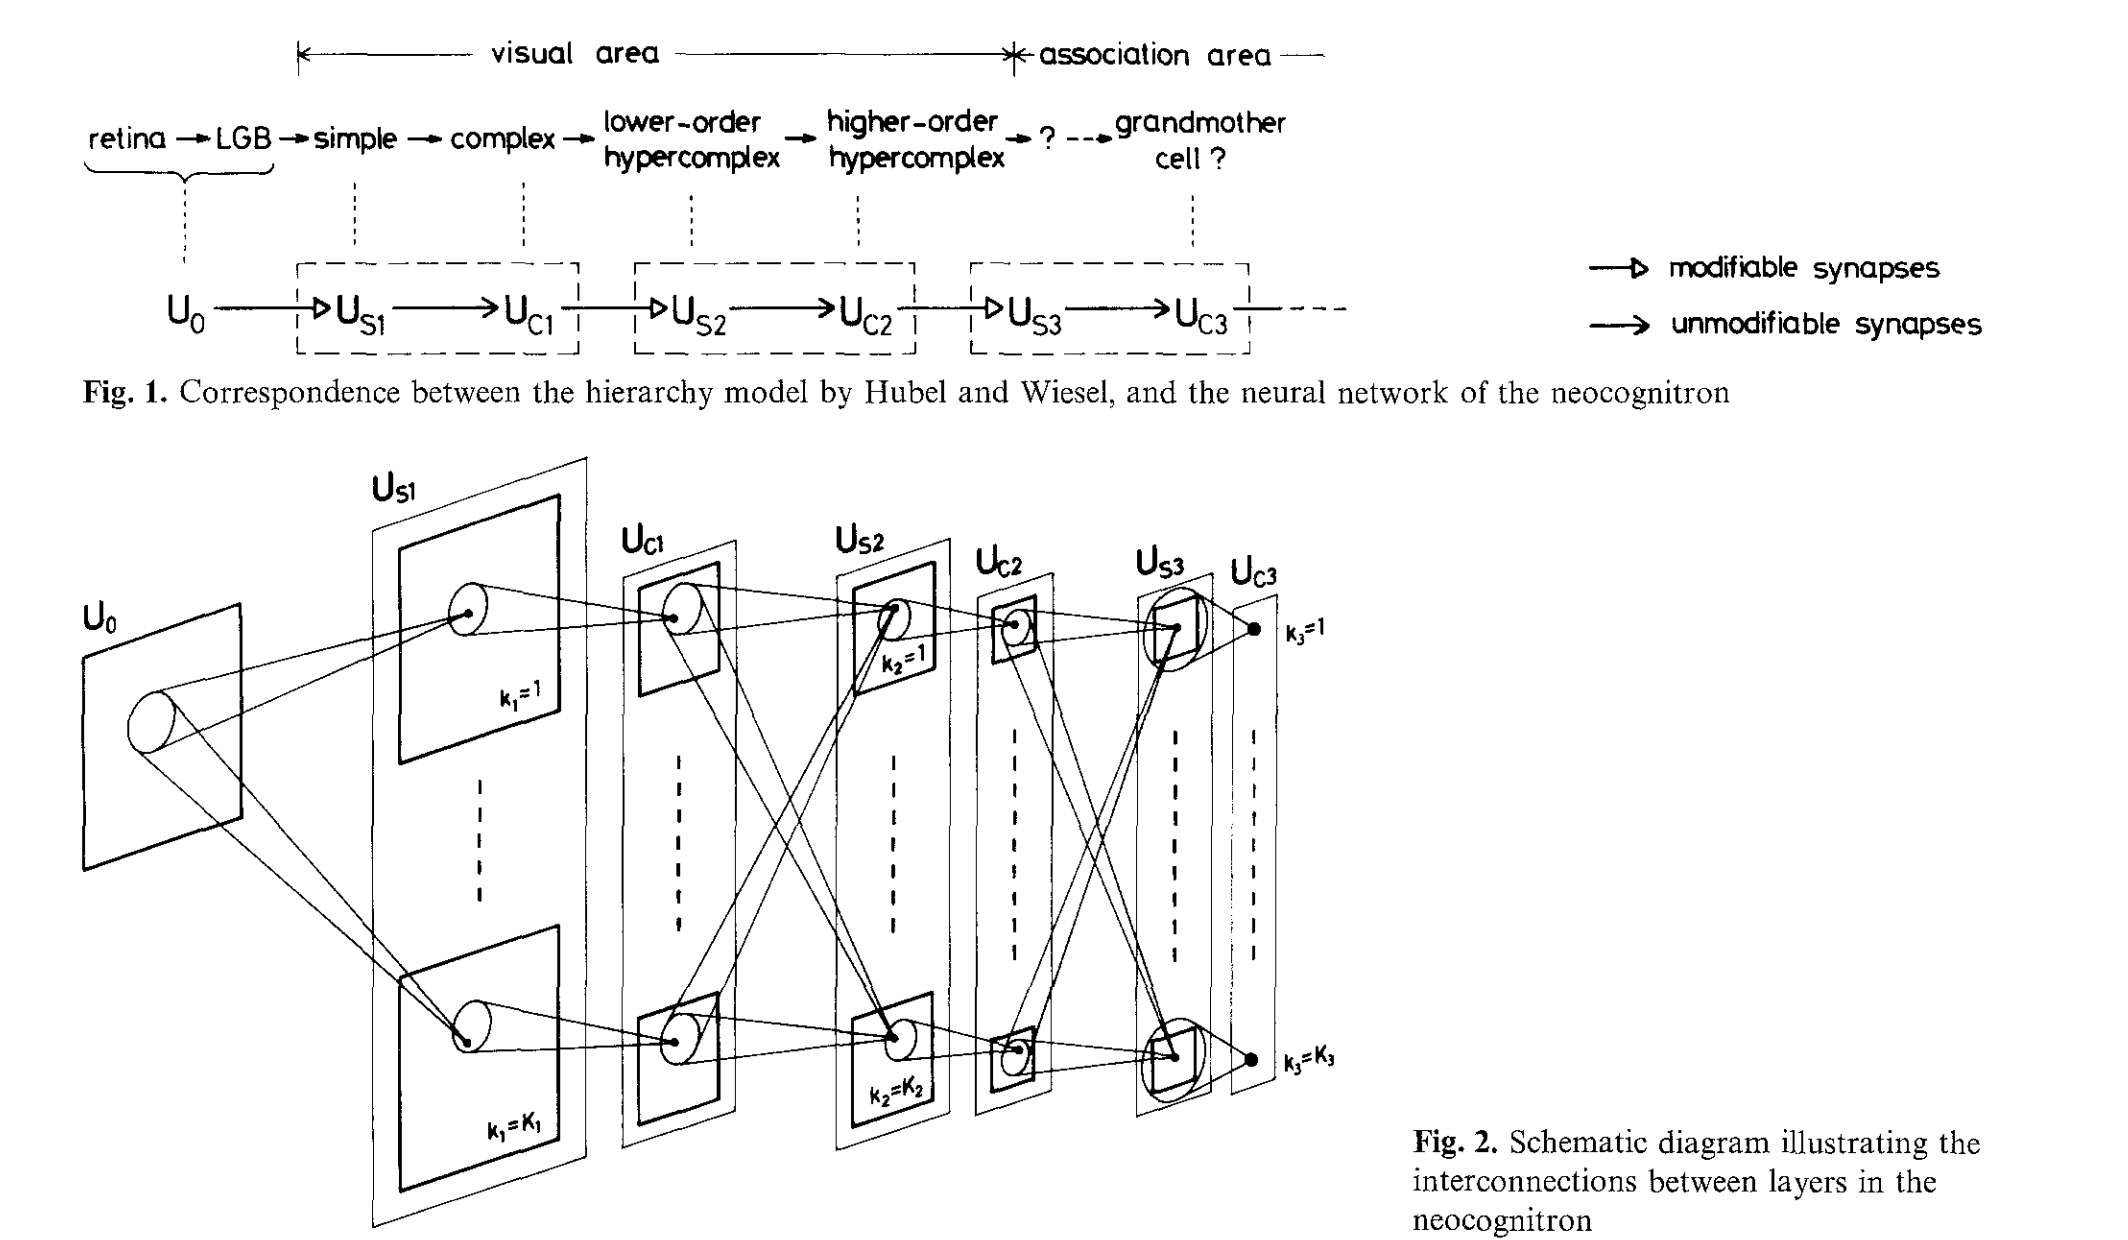
\includegraphics[width=\textwidth]{img/fukushima.png}%
    \caption{Network architecture from Neocognitron.}%
    \label{fig:neocognitron}%
\end{figure}

\subsection{Convolutional neural networks (CNN's)}
Although Neocognitron formed the general idea of the convolutional neural networks, it did not used the method called backpropagation that CNN's use today. Backpropagation is technique used in neural networks to propagate errors through the layers of neural network. First CNN that have the attributes same as current CNN's was build in Bell Labs in 1989 to recognize the hand written digits of the zip codes \cite{cnnzipcodes}. Convolutional neural network name indicates that network uses mathematical operation called \textbf{convolution}. Explaining in a simple way using definition in the Deep Learning book \cite{deeplearningbook}:

\begin{quote}
    "Convolutional networks are simply neural networks that use convolution in place of general matrix multiplication in at least one of their layers."
\end{quote}

Convolutional neural networks are generally a good option for image or time series data problems because of the sliding window approach capturing the underlying signal.

\subsection{Prominent computer vision architectures}
In this project I will be taking advantage of the well known network architectures for computer vision for general benchmarking purposes. These architecture generally known for their good performance in image classification competitions hence, any new design should perform better than these designs to be considered. 

\subsection{LeNet-5}
LeNet-5 \cite{Lenet5} is 7 layered neural network build for classifying hand written digits in checks. Numbers in checks turned into  $32 \times 32$ pixel images and feed into the network for image classification task. LeNet-5 is the first successful application for combination of CNN and backpropagation. Network representation illustration and full specification of the network outlined below.

\begin{figure}[H]%
    \centering
    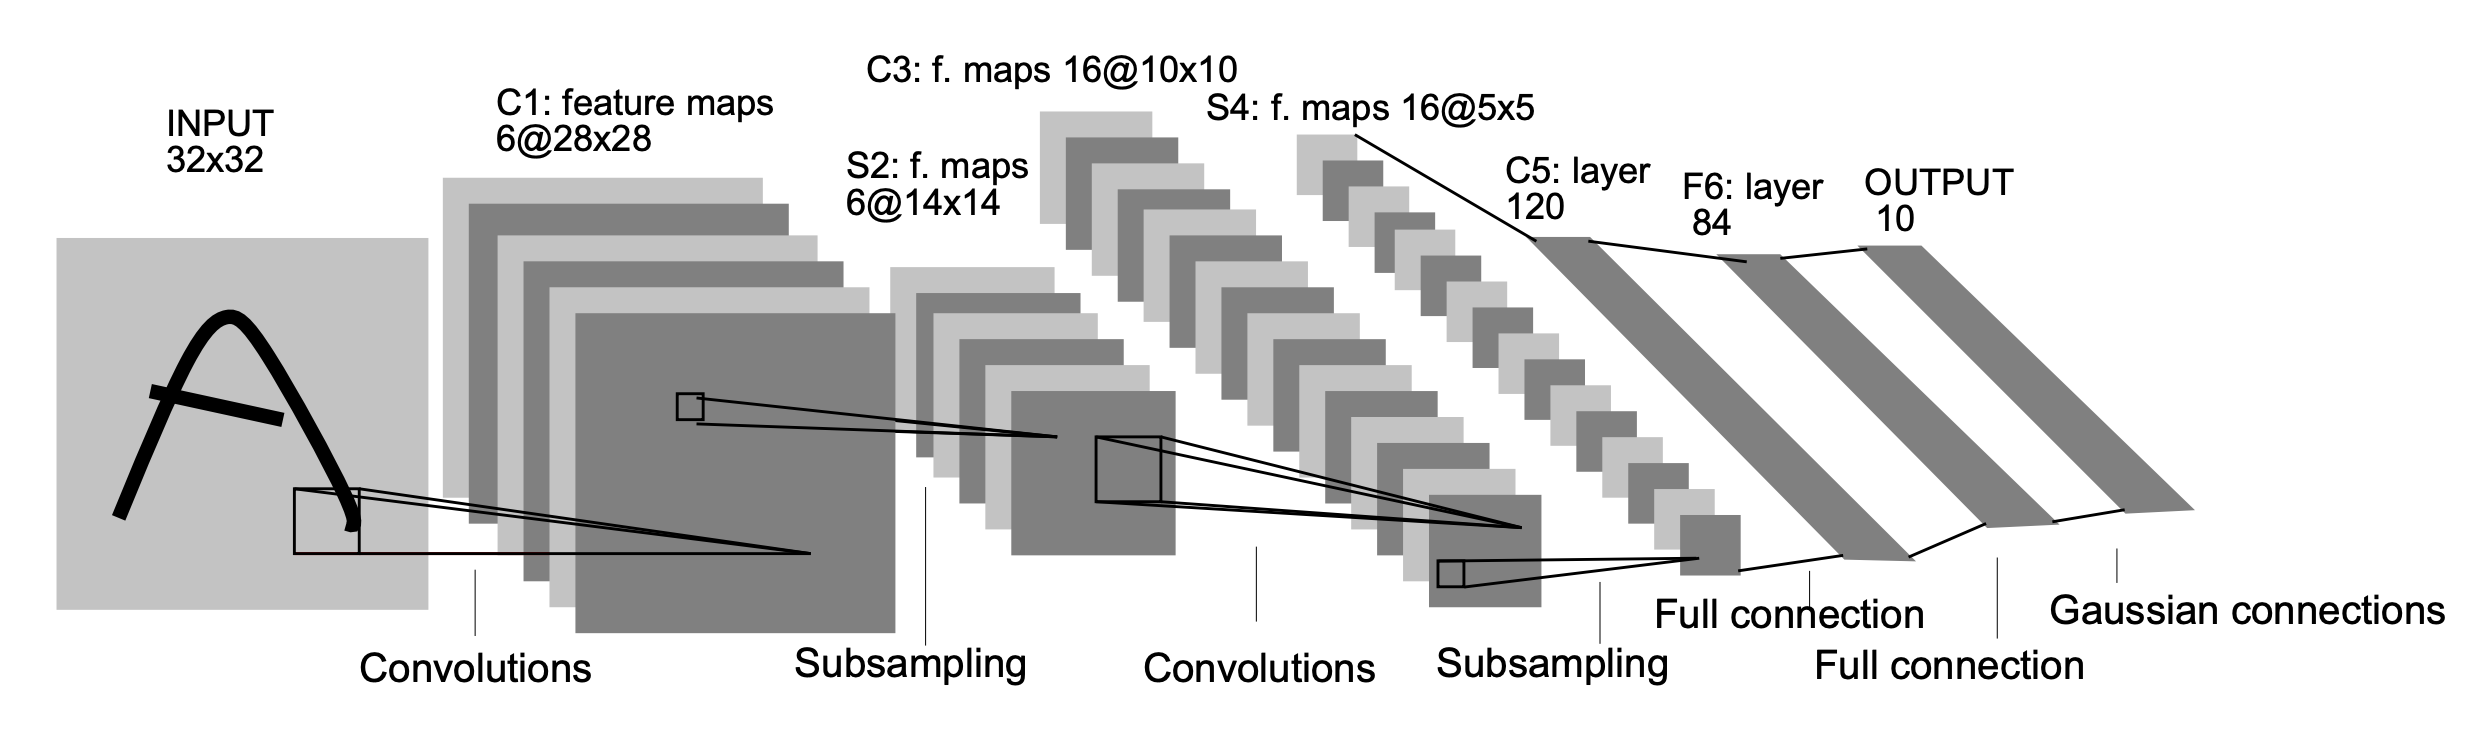
\includegraphics[width=\textwidth]{img/lenet-5.png}%
    \caption{Network architecture of LeNet-5.\\Credit: LeNet-5 \cite{Lenet5}}%
    \label{fig:lenet5}%
\end{figure}


\subsection{AlexNet}
AlexNet \cite{Alexnet} designed and named after Alex Krizhevsky, and published with collaboration of Ilya Sutskever and Geoffrey Hinton (advisor). It was designed for ImageNet challenge \cite{imagenet} and utilized the idea of combining neural networks with graphics processing units (GPU) for high performance. This combination overcome the restriction of high computational demanding nature of neural networks and proved that current computational techniques are sufficient for training neural networks in even very large dataset such as the ImageNet. Another important implication is that AlexNet brought neural networks back to spotlight for research community after long break from LeNet-5's results. 

\begin{figure}[H]%
    \centering
    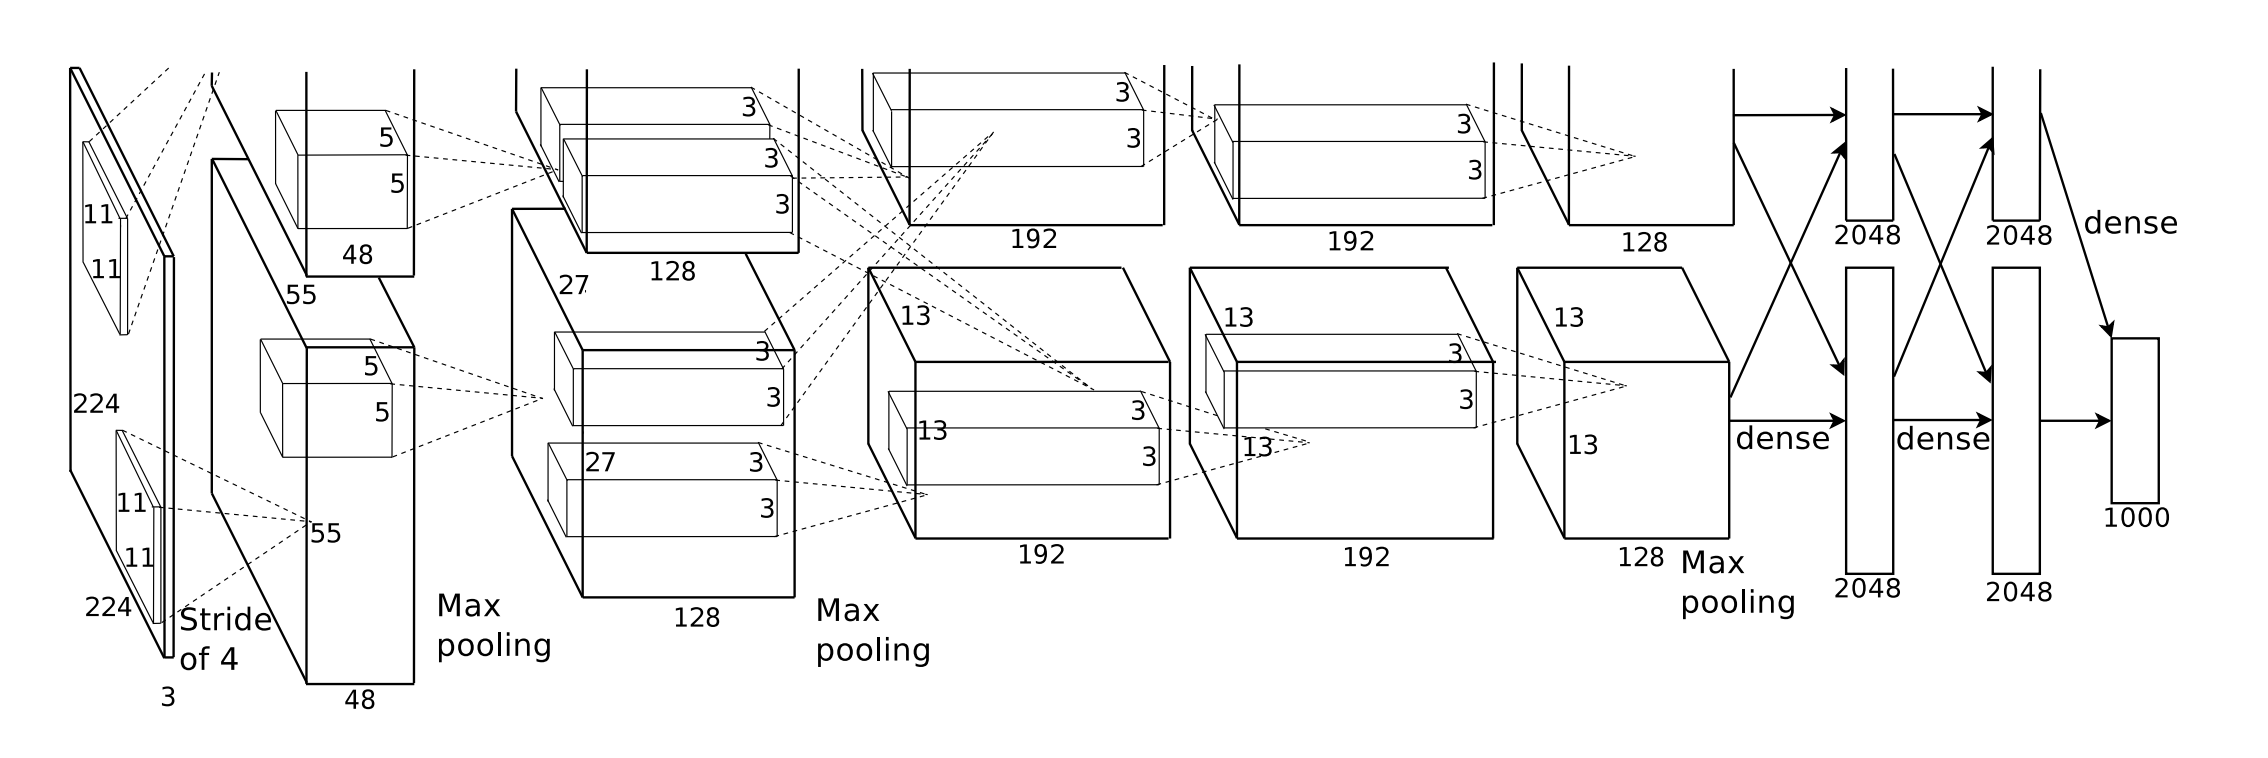
\includegraphics[width=\textwidth]{img/alexnet.png}%
    \caption{Network architecture of AlexNet.\\Credit: AlexNet \cite{Alexnet}}%
    \label{fig:alexnet}%
\end{figure}

\subsection{VGGNet}
VGGNet \cite{vggnet} designed by Visual Geometry Group (VGG) from University of Oxford, this architecture also participated in ImageNet challenge \cite{imagenet} for the year 2014. This research investigated the depth of the convolution neural networks effect on their accuracy. Doing so article walks through their general layout for experimenting different depth and characteristic of neural networks with comparison. Trial error approach they assumed, presents useful methodology for network prototyping this project will use. After obtaining high accuracy from this new deeper neural network inspired many similar high depth neural network architectures to be build. Success of these deep neural networks also get popular which lead the new popular term \textit{Deep Learning}.

\subsection{Computer vision technique for this project}
This section in computer vision intended for short introduction and history of the neural networks. Main reasoning behind this introduction is this project chosen neural networks as primary algorithm for the image classification problem. Reasons for that decision is the achievements of the neural networks withing the machine learning field, specifically within the image classification. So far neural network approach achieved near human level image classification, speech recognition, machine translation and more. Although decision to choose neural network for primary method for this project established, classification accuracy will be compered with other machine learning techniques throughout this project.
\clearpage

\section{Project Aim and Objectives}
\subsection{Aim}
\textcolor{blue}{Aim of this project is to build a fully functional chest x-ray image classification pipeline that implements CI/CD principals to experimentation and deployment. Main classification algorithm I will use for this project is the neural networks, specifically convolutional neural networks. Highest possible accuracy will be aimed but due to highly iterative and time consuming nature of the neural network research, its not very likely that it will beat general benchmark set by most recent research.}

\subsection{Objectives}
Project will be implemented with execution of fallowing objectives:
\begin{itemize}
    \color{blue}
    \item \textbf{Carrying out general data exploration: }This part involves general check on dataset.
    \item \textbf{Data pre-processing and augmentation: }Preparing the data for model ready state.
    \item \textbf{Building baseline model with well known neural network architectures: }This step involves setting additional benchmarks with out of the box models from section 3.
    \item \textbf{Using pre-trained network to increase model performance: }Using pre-trained networks to help training and accuracy of the model.
    %\item Model improvement and hyper parameter tuning
    \item \textbf{Visualizing neural network to ensure learning quality: } For making sure model learning as intended and focusing on correct parts of the image.
    \item \textbf{Ensemble different models: }Using ensemble method with different neural network architectures.
    %\item \textbf{Model refinement: } Prototyping for improved model thorough hyper-parameter tuning.
    %\item Saving trained model for deployment
    \item \textbf{Apply different deployment options: } Implementation of different deployment options. Based on their trade offs. 
\end{itemize}
\clearpage


\section{Methodology}
\subsection{General data exploration}
\textcolor{blue}{I will start with high level checks on data. This step involves general data exploration such as checking if there is a class inbalance in the dataset or size and quality related issues in some images.}

\subsection{Data pre-processing and augmentation}
\textcolor{blue}{Many images can have inherent sources of variance that likely to effect the performance of the classification tasks. Some example to these sources of variance are, angle variance, contrast variance and positional variance. Process such as histogram equalization will be apply to images to increase contrast in the images. This process will lead to information difference between bone any different tissues become more prominent. Various image processing tool available in the keras \cite{keras} and scikit-image \cite{skimage} libraries for this processes. 
I will also make use of some classic data augmentation techniques to avoid over-fitting. One of the most common technique is to flip the images left and right also flip them 90, 180 or 270 degrees.}

\subsection{Building baseline model with neural network architecture}
\textcolor{blue}{Apart from using the CheXNet \cite{CheXNetRP} radiologist accuracy benchmark, architectures from section 3 will be trained to set a baseline benchmark accuracy. Because of their well established position in the machine learning field detailed specifications of these architectures are widely available. In fact keras library \cite{keras} have readily available implementation of these models.}

%\subsection{Model improvement and hyper parameter tuning}

\subsection{Using pre-trained neural network to increase model performance}
\textcolor{blue}{A common and effective technique in computer vision is to use pre-trained network to train a new network. This approach especially successful when the dataset is relatively small. Pre-trained network is usually trained in another large scale image classification data such as ImageNet \cite{imagenet}. Features learned from this dataset acts as a high level model and help training of the new network. General way this process works is to keep the convolutional layers (also referred as convolutional base) of the pre-trained network and connect that layers to a dense (fully connected) layer thats not been trained. Then this newly designed network will be trained on the x-ray images.}

\subsection{Visualizing neural network to ensure learning}
\textcolor{blue}{
It is import to visualize the neural net to identify which parts of the image it's emphasize. Wide range of different visualization approaches available for visualizing convolution networks. Two selected approach that to be applied are the fallowing:
\begin{itemize}
    \item \textit{Visualizing intermediate convolution network outputs.} Generally useful for understating how convolution networks transform their input.
    \item \textit{Heatmaps of class activation.} This visualization technique is most relevant to x-ray image classification. It emphasize part of the image identified as member to certain class which is way of localize objects in the image. 
\end{itemize}
}

%\subsection{Saving trained model for deployment}
\subsection{Ensemble different models}
\textcolor{blue}{Ensemble is a classic machine learning method where different models will used together in prediction to gain better result. Main assumption of the ensemble method is independent models will bring different bias to overall prediction where the individual mistakes of the models will be mitigated by the prediction of other models. Effective application of ensemble requires different models to be trained on data and not having simply using different initialization in of the same neural network. In this project different architectures will be trained to form an ensemble model. Method for the ensemble will be averaging and weighted average of the models. In weighted average, weights will chosen based on their accuracy. In other words highly accurate model will be given high weight.}

\subsection{Apply different deployment options}
\textcolor{blue}{This is a very broad topic with many different deployment options and design choices available. It is not possible to cover all available options within the scope of this project. Therefore selected deployment options will be implemented.}

\textcolor{blue}{After the training of model completed project moves proceeds to saving the trained model in standalone file that could be used to make predictions. Most cost effective and computationally cheap option is to let prediction happen in the client side of the user. This can be achieved by using JavaScript in the web page that will be served to end user. All modern browsers support JavaScript code to be run in the browser which will enable code and model prediction to run in users device. This option is within reach of the project due to the software packages like TensorFlow.js \cite{tensorjs} that enables trained model to be converted into JavaScript completable file that will be served in static website. Although this option cheap and easy way to provide smart solutions to everyone, it is not suitable for commercial initiatives due to fact that anyone can extract the trained model from source code of the page and use it without creators knowledge.}

\textcolor{blue}{Most widely used option when it comes to deployment machine learning models is building RESTful API to serve incoming requests from a central server(s).  This deployment will be build using open source server implemented on the cloud. Reason for choosing the RESTful approach is to building system loosely coupled from the front end design and to enable it to be implemented third part systems.}

\section{Tools and Techniques}
For the implementation of the aims of this project python programming language is chosen as a main programming language. Reasons for this decision is two fold, first part of the reasoning is need of high level programming language. Low level programming languages such as Java or C++ are not well suited for computer vision tasks such as this project due to reason of their time consuming prototyping cycles. Second part of the decision python being de facto language of choice for majority users which enables more tools and techniques being available for application. 

I will also make use of external open source machine learning packages because of the intensive computational nature of the Neural networks. Number of parameters for some of the well known neural network architectures reaches to hundreds of thousands or in some cases in millions or billions. Therefore any code that implements these architecture required to be well optimized and preferably parallelized to run in highly performance hardware, such as the GPU units. Building a code base that achieves this standards require significant amount of time and resource, hence out of the scope of this project. 

Open source projects and their intended form of usage in this project fallows:

\begin{itemize}
    \item \textbf{Scikit-Learn \cite{scikit-learn}: }For the well versed library of machine learning algorithms and tolls such as train / test split for dataset.
    \item \textbf{Pandas \cite{pandas}: }For general data manipulation.
    \item \textbf{Tensorflow \cite{tensorflow} or PyTorch \cite{pytorch}: }For the implementation of the neural network.
    \item \textbf{Matplotlib \cite{matplotlib} and Seaborn \cite{seaborn}: }Visualizing data and calculations.
    \item \textbf{Keras \cite{keras}: }Keras will be used to implement benchmark architectures such as LeNet-5 or AlexNet for the ease of prototyping.
\end{itemize}
\clearpage

\section{Project Plan}
\textcolor{blue}{Fallowing task are based on the project objectives that explained in detail in methodology section. Project will begin on June 14th and continue until 16th of September which is deadline for report submission day. } 

\begin{itemize}
    \color{blue}
    \item \textbf{Task 1: }Carrying out general data exploration. (1 - 2 days)
    \item \textbf{Task 2: }Data pre-processing and augmentation. (2 - 4 days)
    \item \textbf{Task 3: }Building baseline model with well known neural network architectures. (10 - 12 days)
    \item \textbf{Task 4: }Using pre-trained network to increase model performance. (14 - 18 days)
    \item \textbf{Task 5: }Visualizing neural network to ensure learning quality. (9 - 11 days)
    \item \textbf{Task 6: }Ensemble different models. (20 - 24 days)
    \item \textbf{Task 7: }Apply different deployment options. (18 - 22 days)
    \item \textbf{Task 8: }Project Writing (Throughout the project)
\end{itemize}

\noindent\resizebox{\textwidth}{!}{
\begin{ganttchart}[
    title/.append style={fill=black!10},
    title label font=\tiny,
    x unit=4pt,
     time slot format=isodate,
    ]{2019-06-17}{2019-09-15}

    \gantttitlecalendar{year, month=name, week} \\

    \ganttbar{Task 1}{2019-06-18}{2019-06-20} \\
    \ganttbar{Task 2}{2019-06-20}{2019-06-24} \\
    \ganttbar{Task 3}{2019-06-24}{2019-07-06} \\
    \ganttbar{Task 4}{2019-07-06}{2019-07-24} \\
    \ganttbar{Task 5}{2019-07-24}{2019-08-04} \\
    \ganttbar{Task 6}{2019-08-04}{2019-08-28} \\
    \ganttbar{Task 7}{2019-08-24}{2019-09-14} \\
    \ganttbar{Task 8}{2019-06-18}{2019-09-14} \\

%\caption{Timeline of the project tasks.}
\end{ganttchart}
}

\clearpage

\printbibliography
\addcontentsline{toc}{section}{References}

\end{document}